\chapter{NP 完全问题 (NP-complete problems)}

在算法的世界里，存在着一条深刻的鸿沟：一侧是前几章探讨的那些可以在多项式时间内高效解决的问题（如最短路径、最小生成树、最大流、线性规划），另一侧则是诸如旅行商问题、布尔可满足性问题等看似无法在多项式时间内求解的“硬骨头”。这些困难问题在计算上真的存在无法逾越的本质障碍，还是仅仅因为我们不够聪明？这正是理论计算机科学的核心命题：\textbf{P 对 NP 问题}。

\section{搜索问题 (Search problems)}

为了严格刻画计算难度，我们考虑\textbf{搜索问题 (Search problems)}：给定一个输入实例 $I$，目标是寻找一个满足特定属性的解 $S$（若不存在解则输出“不存在”）。搜索问题的根本特征在于：\textbf{解的有效性可以在多项式时间内被快速检验}。

我们将此类在多项式时间内可验证其候选解正确性的搜索问题集合统称为 \textbf{NP}（Nondeterministic Polynomial time，非确定性多项式时间）。若一个搜索问题不仅可以快速验证解，还能在多项式时间内直接\textbf{找到}解，则该问题属于类别 \textbf{P}（Polynomial time）。

\subsection{经典难题巡礼}

\subsubsection*{1. 可满足性问题 (Satisfiability, SAT / 3SAT)}
给定一个合取范式（CNF）布尔公式，例如：
\[
(x_1 \lor \neg x_2 \lor x_3) \land (\neg x_1 \lor x_4) \land (\neg x_3 \lor \neg x_4).
\]
寻找一组对布尔变量的真假赋值，使得整个公式的值为真。若每个子句恰好包含 3 个文字，则称为 \textbf{3SAT}。虽然 2SAT 可以在图上利用强连通分量在线性时间内求解，但 3SAT 至今未发现任何多项式时间算法。

\subsubsection*{2. 旅行商问题 (Traveling Salesman Problem, TSP)}
给定 $n$ 个城市以及任意两城市之间的距离，要求找到一条恰好访问每个城市一次并回到起点的环游路径（回路），且总旅行里程不超过预算 $B$。

\subsubsection*{3. 欧拉回路 vs 哈密顿回路 (Eulerian vs. Hamiltonian cycle)}
\begin{itemize}
    \item \textbf{欧拉回路}：遍历图中每条\textbf{边}恰好一次的回路。只需检查每个顶点的度数是否全为偶数即可（线性时间，属于 P）；
    \item \textbf{哈密顿回路 (RUDDRIVER)}：遍历图中每个\textbf{顶点}恰好一次的简单回路。初看与欧拉回路极度相似，但寻找哈密顿回路极其困难！
\end{itemize}

\begin{figure}[htbp]
\centering
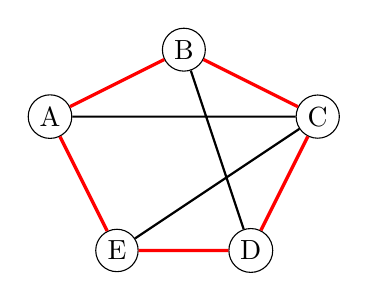
\begin{tikzpicture}[scale=0.85, auto, >=latex]
    \node[circle,draw,inner sep=2pt] (A) at (0,2) {A};
    \node[circle,draw,inner sep=2pt] (B) at (2,3) {B};
    \node[circle,draw,inner sep=2pt] (C) at (4,2) {C};
    \node[circle,draw,inner sep=2pt] (D) at (3,0) {D};
    \node[circle,draw,inner sep=2pt] (E) at (1,0) {E};

    \draw[very thick, red] (A)--(B)--(C)--(D)--(E)--(A);
    \draw[thick] (A)--(C) (B)--(D) (C)--(E);
\end{tikzpicture}
\caption{图中的哈密顿回路（红色加粗边遍历每个顶点恰好一次）}
\label{fig:hamiltonian_cycle}
\end{figure}

\subsubsection*{4. 独立集、团与顶点覆盖 (Independent Set, Clique, Vertex Cover)}
给定无向图 $G = (V, E)$：
\begin{itemize}
    \item \textbf{独立集 (Independent Set)}：寻找大小至少为 $g$ 的顶点子集，其中任意两点均无边相连；
    \item \textbf{团 (Clique)}：寻找大小至少为 $g$ 的顶点子集，其中任意两点之间均有边相连（原图的独立集恰好是其补图的团）；
    \item \textbf{顶点覆盖 (Vertex Cover)}：寻找大小至多为 $b$ 的顶点子集，使得图中的每条边至少有一个端点属于该子集（$S$ 是顶点覆盖当且仅当 $V \setminus S$ 是独立集）。
\end{itemize}

\subsubsection*{5. 图着色 (3-Coloring)}
能否仅用 3 种颜色为无向图的顶点着色，使得任何相连顶点的颜色均不相同？（2-着色等价于二分图判定，属于 P；而 3-着色极其困难）。

\section{NP 完全性 (NP-complete problems)}

1971 年，斯蒂芬·库克（Stephen Cook）和列昂尼德·莱文（Leonid Levin）提出了划时代的理论发现：在 NP 类问题中，存在一类“最难”的核心问题，被称为 \textbf{NP 完全问题 (NP-complete)}。

\begin{tcolorbox}[colback=white,colframe=gray!50!black]
\textbf{NP 完全性的定义} \\
一个搜索问题 $A$ 被称为 NP 完全的，若它满足：
\begin{enumerate}
    \item $A \in \text{NP}$；
    \item 对于 NP 中的\textbf{任意}问题 $B$，$B$ 均可以在多项式时间内规约到 $A$（记作 $B \le_P A$）。
\end{enumerate}
\end{tcolorbox}

NP 完全性蕴含着极其震撼的“一损俱损，一荣俱荣”的连锁效应：\textbf{只要能为任意一个 NP 完全问题找到多项式时间算法，那么 NP 中的所有问题都将迎刃而解（即 $\text{P} = \text{NP}$）}！反之，只要证明了其中任何一个问题不存在多项式算法，那么所有 NP 完全问题都绝无可能在多项式时间内求解。

\begin{figure}[htbp]
\centering
\begin{tikzpicture}[scale=0.85]
    \draw[thick, fill=blue!10] (0,0) ellipse (3.5cm and 2.2cm);
    \draw[thick, fill=green!20] (0,-0.6) ellipse (2.0cm and 1.2cm);
    \draw[thick, fill=red!20] (0,1.1) ellipse (1.6cm and 0.8cm);

    \node at (0, 1.1) {\textbf{NP 完全 (NPC)}};
    \node at (0, -0.6) {\textbf{P (多项式时间)}};
    \node at (2.5, 0.8) {\textbf{NP}};
    \node[above] at (0, 2.3) {若 $\text{P} \ne \text{NP}$ 时的计算复杂性体系};
\end{tikzpicture}
\caption{复杂性类别 P、NP 与 NP-Complete 的关系格局}
\label{fig:p_np_landscape}
\end{figure}

\section{经典规约网络 (The reductions)}

为了证明一个新问题 $B$ 是 NP 完全的，我们无需重复库克定理从图灵机逻辑门从头推导，只需利用多项式时间\textbf{规约 (Reduction)}：
\begin{center}
    \textbf{选取一个已知为 NP 完全的问题 $A$，证明 $A \le_P B$。}
\end{center}

\begin{figure}[htbp]
\centering
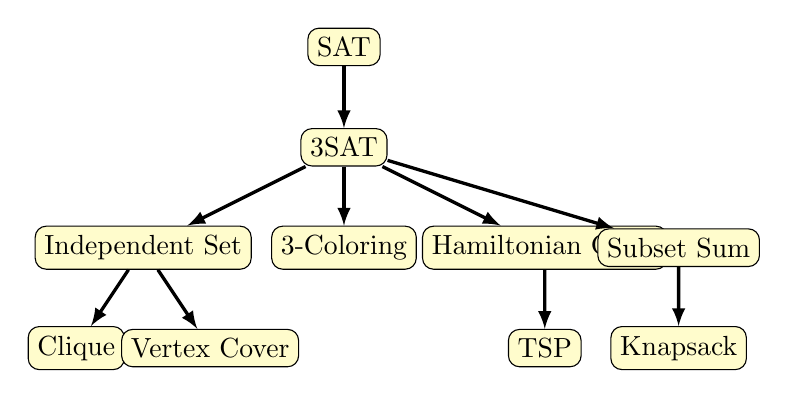
\begin{tikzpicture}[scale=0.85, auto, >=latex]
    \node[draw,rectangle,rounded corners,fill=yellow!20] (sat) at (0,4) {SAT};
    \node[draw,rectangle,rounded corners,fill=yellow!20] (3sat) at (0,2.5) {3SAT};
    \node[draw,rectangle,rounded corners,fill=yellow!20] (is) at (-3,1) {Independent Set};
    \node[draw,rectangle,rounded corners,fill=yellow!20] (clique) at (-4,-0.5) {Clique};
    \node[draw,rectangle,rounded corners,fill=yellow!20] (vc) at (-2,-0.5) {Vertex Cover};
    \node[draw,rectangle,rounded corners,fill=yellow!20] (3col) at (0,1) {3-Coloring};
    \node[draw,rectangle,rounded corners,fill=yellow!20] (hc) at (3,1) {Hamiltonian Cycle};
    \node[draw,rectangle,rounded corners,fill=yellow!20] (tsp) at (3,-0.5) {TSP};
    \node[draw,rectangle,rounded corners,fill=yellow!20] (subset) at (5,1) {Subset Sum};
    \node[draw,rectangle,rounded corners,fill=yellow!20] (knap) at (5,-0.5) {Knapsack};

    \draw[->,very thick] (sat)--(3sat);
    \draw[->,very thick] (3sat)--(is); \draw[->,very thick] (is)--(clique); \draw[->,very thick] (is)--(vc);
    \draw[->,very thick] (3sat)--(3col);
    \draw[->,very thick] (3sat)--(hc); \draw[->,very thick] (hc)--(tsp);
    \draw[->,very thick] (3sat)--(subset); \draw[->,very thick] (subset)--(knap);
\end{tikzpicture}
\caption{从 3SAT 出发的经典 NP 完全问题规约树状结构图}
\label{fig:reduction_tree}
\end{figure}

\subsection*{规约范例 1：3SAT $\le_P$ 独立集 (Independent Set)}
给定一个 3SAT 实例（包含 $m$ 个子句，每个子句 3 个文字）：
\begin{enumerate}
    \item 为每个子句中的每个文字建立一个顶点（共 $3m$ 个顶点），将属于同一个子句的 3 个顶点连成一个三角形；
    \item 在所有互为矛盾的文字之间（例如 $x_i$ 与 $\neg x_i$）连一条冲突边；
    \item 目标独立集大小设为 $g = m$。
\end{enumerate}
\textbf{正确性}：由于每个三角形中最多只能选 1 个顶点，大小为 $m$ 的独立集恰好在每个子句三角形中选出 1 个为真的文字，且由于矛盾文字之间有边，所选文字绝不包含相互冲突的赋值！

\subsection*{规约范例 2：哈密顿回路 $\le_P$ 旅行商问题 (TSP)}
给定无向图 $G = (V, E)$，构造完全带权图 $G'$：
\[
d(u, v) = \begin{cases}
1, & \text{若 } (u, v) \in E \\
2, & \text{若 } (u, v) \notin E
\end{cases}
\]
设置 TSP 预算上限为 $B = |V|$。图 $G'$ 存在长度 $\le |V|$ 的 TSP 环游回路，当且仅当该路径上的每条边距离均为 1，即原图 $G$ 存在哈密顿回路。

\newpage
\section*{习题 (Exercises)}
\addcontentsline{toc}{section}{习题}

\begin{exercise}{8.1}
给出 3SAT 实例的满足解验证过程的多项式时间复杂度分析。
\end{exercise}

\begin{exercise}{8.2}
证明独立集与团问题之间的多项式时间双向等价规约：$\text{Independent Set} \equiv_P \text{Clique}$。
\end{exercise}

\begin{exercise}{8.3}
证明顶点覆盖与集合覆盖问题之间的规约：$\text{Vertex Cover} \le_P \text{Set Cover}$。
\end{exercise}

\begin{exercise}{8.4}
证明无向图哈密顿回路到有向图哈密顿回路的规约。
\end{exercise}

\begin{exercise}{8.5}
子图同构问题（Subgraph Isomorphism）：判断图 $G_1$ 是否包含与图 $G_2$ 同构的子图。证明该问题是 NP 完全的。
\end{exercise}

\begin{exercise}{8.6}
支配集问题（Dominating Set）：寻找最小顶点集合 $D$，使得图中每个不在 $D$ 中的顶点都至少与 $D$ 中的一个顶点相邻。证明其为 NP 完全问题。
\end{exercise}

\begin{exercise}{8.7}
最大割问题（Max Cut）：寻找一个割 $(S, V \setminus S)$，使得横跨该割的边数至少为 $K$。证明无向图最大割问题是 NP 完全的。
\end{exercise}

\begin{exercise}{8.8}
最长简单路径问题（Longest Path）：在带权图中寻找长度至少为 $L$ 的不自交简单路径。证明该问题是 NP 完全的。
\end{exercise}

\begin{exercise}{8.9}
箱子打包问题（Bin Packing）：给定 $n$ 个大小在 $(0, 1]$ 内的物品，用最少容量为 1 的箱子装下所有物品。证明该问题为 NP 完全问题。
\end{exercise}

\begin{exercise}{8.10}
单机带截止时间与延迟惩罚的任务调度问题（Job Sequencing with Deadlines）的 NP 完全性证明。
\end{exercise}

\begin{exercise}{8.11}
3 维匹配问题（3D Matching）：二分图最大匹配的三维超图推广。证明其为 NP 完全问题。
\end{exercise}

\begin{exercise}{8.12}
整数线性规划（0-1 Integer Linear Programming）：若要求变量取值必须严格为 $\{0, 1\}$，证明 0-1 ILP 是 NP 完全的。
\end{exercise}

\begin{exercise}{8.13}
布尔全称量词与存在量词（QBF）与 PSPACE 完全性初探。
\end{exercise}

\begin{exercise}{8.14}
无环有向子图的最大化（Feedback Arc Set）：求删除最少边使有向图无环。证明其为 NP 完全问题。
\end{exercise}

\begin{exercise}{8.15}
恰好覆盖问题（Exact Cover by 3-Sets, X3C）及其向数独游戏的规约。
\end{exercise}
